\clearpage\appendix

\section{Question-Level Audit Tables}
\label{app:audit}

The following tables report per-question correctness and evidence recall for BM25 (baseline arm)
and the deployed hybrid selector (enhanced arm) at all three evaluated token budgets.
Correctness and evidence recall are majority-vote aggregates over three answering calls per question
per selector. A value of~1 indicates that the majority of calls produced a correct answer or
delivered the required evidence; 0 indicates the majority did not. These are single-run outcomes
and are not independent replications across budgets. Question IDs are truncated to 22 characters
for readability; full IDs are available in the raw records.

\begin{table}[htbp]\centering\small
\caption{Paired outcome summary across all three token budgets. BM25-only and Hybrid-only count questions where only that selector answers correctly. CTLS values are conservative lower bounds derived from existing selector records.}
\label{tab:outcome_summary}
\begin{tabular}{lrrrrrrrrr}\toprule
Budget & $N$ & BM25 & Hyb & HNT & CTLS* & Both(BM25+Hyb) & BM25-only & Hyb-only & Neither \\\midrule
512 tok  & 84 & 57(67\%) & 27(32\%) & 48(57\%) & 65(77\%) & 22 & 35 & 5 & 22 \\
1024 tok & 84 & 55(65\%) & 30(35\%) & 53(63\%) & 65(77\%) & 20 & 35 & 10 & 19 \\
2048 tok & 84 & 58(69\%) & 30(35\%) & 59(70\%) & 67(80\%) & 24 & 34 & 6 & 20 \\
\bottomrule\end{tabular}
\par\vspace{2pt}\small{* CTLS correct-answer counts are conservative lower bounds: $\max(\text{Jaccard},\text{BM25})$ per question.}
\end{table}

\FloatBarrier

\subsection{Per-question audit: 512-token budget}

\begin{longtable}{@{}clcccc@{}}
\caption{Question-level audit at the 512-token budget. BA = BM25 Answer, BE = BM25 Evidence, HA = Hybrid Answer, HE = Hybrid Evidence. 1 = correct or recalled (majority vote across repeats), 0 = otherwise.}\\
\label{tab:audit_512}\\
\toprule
Row & Question ID & BA & BE & HA & HE \\
\midrule
\endfirsthead
\multicolumn{6}{c}{{\itshape Table \thetable{} continued}} \\[2pt]
\toprule Row & Question ID & BA & BE & HA & HE \\ \midrule
\endhead
\midrule \multicolumn{6}{r}{{\itshape Continued on next page}} \\
\endfoot
\bottomrule
\endlastfoot
Q01 & \texttt{001be529} & 1 & 1 & 0 & 0 \\
Q02 & \texttt{06f04340} & 0 & 1 & 0 & 0 \\
Q03 & \texttt{0862e8bf\_abs} & 1 & 0 & 1 & 0 \\
Q04 & \texttt{09ba9854\_abs} & 1 & 0 & 1 & 0 \\
Q05 & \texttt{09d032c9} & 0 & 0 & 0 & 0 \\
Q06 & \texttt{0ddfec37\_abs} & 1 & 0 & 1 & 0 \\
Q07 & \texttt{0edc2aef} & 0 & 1 & 0 & 0 \\
Q08 & \texttt{0f05491a} & 0 & 1 & 0 & 1 \\
Q09 & \texttt{10e09553} & 1 & 1 & 0 & 0 \\
Q10 & \texttt{1192316e} & 1 & 1 & 0 & 0 \\
Q11 & \texttt{157a136e} & 0 & 1 & 1 & 1 \\
Q12 & \texttt{18dcd5a5} & 1 & 1 & 0 & 0 \\
Q13 & \texttt{19b5f2b3\_abs} & 1 & 0 & 1 & 0 \\
Q14 & \texttt{1b9b7252} & 1 & 1 & 0 & 0 \\
Q15 & \texttt{1c0ddc50} & 0 & 1 & 0 & 0 \\
Q16 & \texttt{1d4e3b97} & 0 & 1 & 0 & 1 \\
Q17 & \texttt{1da05512} & 0 & 1 & 1 & 0 \\
Q18 & \texttt{1e043500} & 1 & 1 & 0 & 0 \\
Q19 & \texttt{2133c1b5\_abs} & 1 & 0 & 1 & 0 \\
Q20 & \texttt{2311e44b\_abs} & 1 & 0 & 1 & 0 \\
Q21 & \texttt{2698e78f} & 1 & 1 & 0 & 0 \\
Q22 & \texttt{28bcfaac} & 1 & 1 & 0 & 0 \\
Q23 & \texttt{29f2956b\_abs} & 1 & 0 & 1 & 0 \\
Q24 & \texttt{2c63a862} & 0 & 1 & 0 & 0 \\
Q25 & \texttt{311778f1} & 1 & 1 & 0 & 0 \\
Q26 & \texttt{37d43f65} & 1 & 1 & 0 & 0 \\
Q27 & \texttt{38146c39} & 0 & 1 & 0 & 0 \\
Q28 & \texttt{3a704032} & 0 & 0 & 0 & 0 \\
Q29 & \texttt{3fe836c9} & 1 & 1 & 0 & 0 \\
Q30 & \texttt{488d3006} & 1 & 1 & 1 & 1 \\
Q31 & \texttt{54026fce} & 1 & 1 & 1 & 0 \\
Q32 & \texttt{5a4f22c0} & 1 & 1 & 1 & 1 \\
Q33 & \texttt{5c40ec5b} & 0 & 1 & 0 & 1 \\
Q34 & \texttt{65240037} & 1 & 1 & 0 & 0 \\
Q35 & \texttt{6a1eabeb} & 1 & 1 & 1 & 1 \\
Q36 & \texttt{6aeb4375\_abs} & 1 & 0 & 1 & 0 \\
Q37 & \texttt{6e984301} & 1 & 1 & 0 & 1 \\
Q38 & \texttt{6f9b354f} & 1 & 1 & 0 & 0 \\
Q39 & \texttt{7161e7e2} & 1 & 1 & 0 & 0 \\
Q40 & \texttt{726462e0} & 1 & 1 & 0 & 0 \\
Q41 & \texttt{72e3ee87} & 1 & 1 & 1 & 1 \\
Q42 & \texttt{8cf51dda} & 1 & 1 & 0 & 0 \\
Q43 & \texttt{8ebdbe50} & 1 & 1 & 0 & 0 \\
Q44 & \texttt{95228167} & 1 & 0 & 0 & 0 \\
Q45 & \texttt{993da5e2} & 1 & 1 & 0 & 1 \\
Q46 & \texttt{9aaed6a3} & 0 & 1 & 0 & 0 \\
Q47 & \texttt{9bbe84a2} & 1 & 1 & 0 & 0 \\
Q48 & \texttt{afdc33df} & 0 & 1 & 0 & 0 \\
Q49 & \texttt{b0479f84} & 1 & 1 & 0 & 0 \\
Q50 & \texttt{b320f3f8} & 1 & 1 & 0 & 0 \\
Q51 & \texttt{ba358f49} & 0 & 1 & 0 & 0 \\
Q52 & \texttt{ba358f49\_abs} & 1 & 0 & 1 & 0 \\
Q53 & \texttt{bc8a6e93\_abs} & 1 & 0 & 1 & 0 \\
Q54 & \texttt{c2ac3c61} & 1 & 1 & 0 & 1 \\
Q55 & \texttt{c4ea545c} & 0 & 1 & 0 & 0 \\
Q56 & \texttt{c4f10528} & 0 & 1 & 0 & 0 \\
Q57 & \texttt{c6853660} & 1 & 1 & 0 & 0 \\
Q58 & \texttt{c960da58} & 1 & 1 & 0 & 0 \\
Q59 & \texttt{caf9ead2} & 1 & 1 & 0 & 0 \\
Q60 & \texttt{cc539528} & 1 & 1 & 1 & 0 \\
Q61 & \texttt{cc5ded98} & 1 & 1 & 0 & 0 \\
Q62 & \texttt{d52b4f67} & 1 & 1 & 0 & 1 \\
Q63 & \texttt{d6233ab6} & 0 & 0 & 0 & 0 \\
Q64 & \texttt{d7c942c3} & 1 & 1 & 0 & 0 \\
Q65 & \texttt{d851d5ba} & 0 & 1 & 0 & 0 \\
Q66 & \texttt{dc439ea3} & 1 & 1 & 0 & 0 \\
Q67 & \texttt{e01b8e2f} & 1 & 1 & 1 & 0 \\
Q68 & \texttt{e982271f} & 1 & 1 & 1 & 0 \\
Q69 & \texttt{edced276\_abs} & 1 & 0 & 1 & 0 \\
Q70 & \texttt{eeda8a6d} & 1 & 1 & 0 & 0 \\
Q71 & \texttt{eeda8a6d\_abs} & 1 & 0 & 1 & 0 \\
Q72 & \texttt{efc3f7c2} & 1 & 1 & 0 & 0 \\
Q73 & \texttt{fca762bc} & 1 & 1 & 0 & 0 \\
Q74 & \texttt{gpt4\_15e38248} & 0 & 0 & 0 & 0 \\
Q75 & \texttt{gpt4\_18c2b244} & 0 & 1 & 1 & 1 \\
Q76 & \texttt{gpt4\_1d80365e} & 1 & 1 & 1 & 1 \\
Q77 & \texttt{gpt4\_213fd887} & 0 & 1 & 1 & 1 \\
Q78 & \texttt{gpt4\_4fc4f797} & 1 & 1 & 1 & 1 \\
Q79 & \texttt{gpt4\_59c863d7} & 0 & 1 & 0 & 0 \\
Q80 & \texttt{gpt4\_8c8961ae} & 0 & 1 & 0 & 1 \\
Q81 & \texttt{gpt4\_d6585ce8} & 0 & 0 & 0 & 0 \\
Q82 & \texttt{gpt4\_ec93e27f} & 1 & 1 & 0 & 1 \\
Q83 & \texttt{gpt4\_f420262c} & 0 & 0 & 0 & 0 \\
Q84 & \texttt{gpt4\_fa19884d} & 0 & 1 & 1 & 0 \\
\end{longtable}

\clearpage

\subsection{Per-question audit: 1024-token budget}

\begin{longtable}{@{}clcccc@{}}
\caption{Question-level audit at the 1024-token budget. BA = BM25 Answer, BE = BM25 Evidence, HA = Hybrid Answer, HE = Hybrid Evidence. 1 = correct or recalled (majority vote across repeats), 0 = otherwise.}\\
\label{tab:audit_1024}\\
\toprule
Row & Question ID & BA & BE & HA & HE \\
\midrule
\endfirsthead
\multicolumn{6}{c}{{\itshape Table \thetable{} continued}} \\[2pt]
\toprule Row & Question ID & BA & BE & HA & HE \\ \midrule
\endhead
\midrule \multicolumn{6}{r}{{\itshape Continued on next page}} \\
\endfoot
\bottomrule
\endlastfoot
Q01 & \texttt{001be529} & 1 & 1 & 0 & 0 \\
Q02 & \texttt{06f04340} & 0 & 0 & 0 & 0 \\
Q03 & \texttt{0862e8bf\_abs} & 1 & 0 & 1 & 0 \\
Q04 & \texttt{09ba9854\_abs} & 0 & 0 & 1 & 0 \\
Q05 & \texttt{09d032c9} & 0 & 0 & 0 & 0 \\
Q06 & \texttt{0ddfec37\_abs} & 1 & 0 & 1 & 0 \\
Q07 & \texttt{0edc2aef} & 1 & 1 & 0 & 0 \\
Q08 & \texttt{0f05491a} & 0 & 1 & 0 & 1 \\
Q09 & \texttt{10e09553} & 1 & 1 & 0 & 1 \\
Q10 & \texttt{1192316e} & 1 & 1 & 0 & 0 \\
Q11 & \texttt{157a136e} & 0 & 1 & 1 & 1 \\
Q12 & \texttt{18dcd5a5} & 1 & 1 & 0 & 0 \\
Q13 & \texttt{19b5f2b3\_abs} & 1 & 0 & 1 & 0 \\
Q14 & \texttt{1b9b7252} & 1 & 1 & 0 & 0 \\
Q15 & \texttt{1c0ddc50} & 1 & 1 & 0 & 0 \\
Q16 & \texttt{1d4e3b97} & 0 & 1 & 0 & 1 \\
Q17 & \texttt{1da05512} & 0 & 1 & 1 & 0 \\
Q18 & \texttt{1e043500} & 1 & 1 & 0 & 0 \\
Q19 & \texttt{2133c1b5\_abs} & 1 & 0 & 1 & 0 \\
Q20 & \texttt{2311e44b\_abs} & 1 & 0 & 1 & 0 \\
Q21 & \texttt{2698e78f} & 1 & 1 & 0 & 1 \\
Q22 & \texttt{28bcfaac} & 1 & 1 & 1 & 0 \\
Q23 & \texttt{29f2956b\_abs} & 1 & 0 & 1 & 0 \\
Q24 & \texttt{2c63a862} & 0 & 1 & 0 & 0 \\
Q25 & \texttt{311778f1} & 1 & 1 & 0 & 0 \\
Q26 & \texttt{37d43f65} & 1 & 1 & 0 & 0 \\
Q27 & \texttt{38146c39} & 0 & 1 & 1 & 0 \\
Q28 & \texttt{3a704032} & 0 & 0 & 0 & 0 \\
Q29 & \texttt{3fe836c9} & 1 & 1 & 0 & 0 \\
Q30 & \texttt{488d3006} & 1 & 1 & 1 & 1 \\
Q31 & \texttt{54026fce} & 0 & 1 & 1 & 0 \\
Q32 & \texttt{5a4f22c0} & 1 & 1 & 1 & 1 \\
Q33 & \texttt{5c40ec5b} & 0 & 1 & 0 & 1 \\
Q34 & \texttt{65240037} & 1 & 1 & 0 & 0 \\
Q35 & \texttt{6a1eabeb} & 1 & 1 & 1 & 1 \\
Q36 & \texttt{6aeb4375\_abs} & 1 & 0 & 1 & 0 \\
Q37 & \texttt{6e984301} & 0 & 1 & 0 & 1 \\
Q38 & \texttt{6f9b354f} & 1 & 1 & 0 & 0 \\
Q39 & \texttt{7161e7e2} & 1 & 1 & 0 & 0 \\
Q40 & \texttt{726462e0} & 1 & 1 & 0 & 0 \\
Q41 & \texttt{72e3ee87} & 1 & 1 & 1 & 1 \\
Q42 & \texttt{8cf51dda} & 1 & 1 & 0 & 0 \\
Q43 & \texttt{8ebdbe50} & 1 & 1 & 0 & 0 \\
Q44 & \texttt{95228167} & 0 & 0 & 1 & 0 \\
Q45 & \texttt{993da5e2} & 0 & 1 & 0 & 1 \\
Q46 & \texttt{9aaed6a3} & 1 & 1 & 0 & 0 \\
Q47 & \texttt{9bbe84a2} & 1 & 1 & 0 & 0 \\
Q48 & \texttt{afdc33df} & 0 & 1 & 0 & 0 \\
Q49 & \texttt{b0479f84} & 1 & 1 & 0 & 0 \\
Q50 & \texttt{b320f3f8} & 1 & 1 & 0 & 0 \\
Q51 & \texttt{ba358f49} & 0 & 1 & 0 & 0 \\
Q52 & \texttt{ba358f49\_abs} & 1 & 0 & 1 & 0 \\
Q53 & \texttt{bc8a6e93\_abs} & 1 & 0 & 1 & 0 \\
Q54 & \texttt{c2ac3c61} & 1 & 1 & 0 & 1 \\
Q55 & \texttt{c4ea545c} & 0 & 1 & 0 & 0 \\
Q56 & \texttt{c4f10528} & 1 & 1 & 0 & 0 \\
Q57 & \texttt{c6853660} & 1 & 1 & 0 & 0 \\
Q58 & \texttt{c960da58} & 1 & 1 & 0 & 0 \\
Q59 & \texttt{caf9ead2} & 1 & 1 & 0 & 0 \\
Q60 & \texttt{cc539528} & 1 & 1 & 1 & 0 \\
Q61 & \texttt{cc5ded98} & 1 & 1 & 0 & 0 \\
Q62 & \texttt{d52b4f67} & 1 & 1 & 0 & 0 \\
Q63 & \texttt{d6233ab6} & 0 & 0 & 0 & 0 \\
Q64 & \texttt{d7c942c3} & 1 & 1 & 0 & 0 \\
Q65 & \texttt{d851d5ba} & 0 & 1 & 0 & 1 \\
Q66 & \texttt{dc439ea3} & 1 & 1 & 0 & 0 \\
Q67 & \texttt{e01b8e2f} & 1 & 1 & 1 & 0 \\
Q68 & \texttt{e982271f} & 1 & 1 & 1 & 0 \\
Q69 & \texttt{edced276\_abs} & 1 & 0 & 1 & 0 \\
Q70 & \texttt{eeda8a6d} & 0 & 1 & 0 & 0 \\
Q71 & \texttt{eeda8a6d\_abs} & 1 & 0 & 1 & 0 \\
Q72 & \texttt{efc3f7c2} & 1 & 1 & 0 & 0 \\
Q73 & \texttt{fca762bc} & 1 & 1 & 0 & 0 \\
Q74 & \texttt{gpt4\_15e38248} & 0 & 0 & 0 & 0 \\
Q75 & \texttt{gpt4\_18c2b244} & 1 & 1 & 1 & 1 \\
Q76 & \texttt{gpt4\_1d80365e} & 0 & 1 & 1 & 1 \\
Q77 & \texttt{gpt4\_213fd887} & 0 & 1 & 1 & 1 \\
Q78 & \texttt{gpt4\_4fc4f797} & 1 & 1 & 0 & 1 \\
Q79 & \texttt{gpt4\_59c863d7} & 0 & 1 & 0 & 0 \\
Q80 & \texttt{gpt4\_8c8961ae} & 1 & 1 & 0 & 1 \\
Q81 & \texttt{gpt4\_d6585ce8} & 0 & 0 & 0 & 0 \\
Q82 & \texttt{gpt4\_ec93e27f} & 0 & 1 & 1 & 1 \\
Q83 & \texttt{gpt4\_f420262c} & 0 & 1 & 0 & 0 \\
Q84 & \texttt{gpt4\_fa19884d} & 0 & 1 & 1 & 0 \\
\end{longtable}

\clearpage

\subsection{Per-question audit: 2048-token budget}

\begin{longtable}{@{}clcccc@{}}
\caption{Question-level audit at the 2048-token budget. BA = BM25 Answer, BE = BM25 Evidence, HA = Hybrid Answer, HE = Hybrid Evidence. 1 = correct or recalled (majority vote across repeats), 0 = otherwise.}\\
\label{tab:audit_2048}\\
\toprule
Row & Question ID & BA & BE & HA & HE \\
\midrule
\endfirsthead
\multicolumn{6}{c}{{\itshape Table \thetable{} continued}} \\[2pt]
\toprule Row & Question ID & BA & BE & HA & HE \\ \midrule
\endhead
\midrule \multicolumn{6}{r}{{\itshape Continued on next page}} \\
\endfoot
\bottomrule
\endlastfoot
Q01 & \texttt{001be529} & 1 & 1 & 0 & 0 \\
Q02 & \texttt{06f04340} & 0 & 0 & 0 & 0 \\
Q03 & \texttt{0862e8bf\_abs} & 1 & 0 & 1 & 0 \\
Q04 & \texttt{09ba9854\_abs} & 0 & 0 & 1 & 0 \\
Q05 & \texttt{09d032c9} & 0 & 0 & 0 & 0 \\
Q06 & \texttt{0ddfec37\_abs} & 1 & 0 & 1 & 0 \\
Q07 & \texttt{0edc2aef} & 0 & 1 & 0 & 0 \\
Q08 & \texttt{0f05491a} & 0 & 1 & 0 & 1 \\
Q09 & \texttt{10e09553} & 0 & 1 & 1 & 1 \\
Q10 & \texttt{1192316e} & 1 & 1 & 0 & 0 \\
Q11 & \texttt{157a136e} & 0 & 1 & 1 & 1 \\
Q12 & \texttt{18dcd5a5} & 1 & 1 & 0 & 0 \\
Q13 & \texttt{19b5f2b3\_abs} & 1 & 0 & 1 & 0 \\
Q14 & \texttt{1b9b7252} & 1 & 1 & 0 & 0 \\
Q15 & \texttt{1c0ddc50} & 1 & 1 & 0 & 0 \\
Q16 & \texttt{1d4e3b97} & 0 & 1 & 0 & 1 \\
Q17 & \texttt{1da05512} & 0 & 1 & 1 & 0 \\
Q18 & \texttt{1e043500} & 1 & 1 & 0 & 0 \\
Q19 & \texttt{2133c1b5\_abs} & 1 & 0 & 1 & 0 \\
Q20 & \texttt{2311e44b\_abs} & 1 & 0 & 1 & 0 \\
Q21 & \texttt{2698e78f} & 1 & 1 & 0 & 0 \\
Q22 & \texttt{28bcfaac} & 1 & 1 & 1 & 0 \\
Q23 & \texttt{29f2956b\_abs} & 1 & 0 & 1 & 0 \\
Q24 & \texttt{2c63a862} & 0 & 1 & 0 & 0 \\
Q25 & \texttt{311778f1} & 1 & 1 & 0 & 0 \\
Q26 & \texttt{37d43f65} & 1 & 1 & 1 & 0 \\
Q27 & \texttt{38146c39} & 0 & 1 & 0 & 0 \\
Q28 & \texttt{3a704032} & 0 & 1 & 0 & 0 \\
Q29 & \texttt{3fe836c9} & 1 & 1 & 0 & 0 \\
Q30 & \texttt{488d3006} & 1 & 1 & 1 & 1 \\
Q31 & \texttt{54026fce} & 1 & 1 & 0 & 0 \\
Q32 & \texttt{5a4f22c0} & 1 & 1 & 1 & 1 \\
Q33 & \texttt{5c40ec5b} & 0 & 1 & 0 & 1 \\
Q34 & \texttt{65240037} & 1 & 1 & 0 & 0 \\
Q35 & \texttt{6a1eabeb} & 1 & 1 & 1 & 1 \\
Q36 & \texttt{6aeb4375\_abs} & 1 & 0 & 1 & 0 \\
Q37 & \texttt{6e984301} & 1 & 1 & 0 & 1 \\
Q38 & \texttt{6f9b354f} & 1 & 1 & 0 & 0 \\
Q39 & \texttt{7161e7e2} & 1 & 1 & 0 & 0 \\
Q40 & \texttt{726462e0} & 1 & 1 & 0 & 0 \\
Q41 & \texttt{72e3ee87} & 1 & 1 & 1 & 1 \\
Q42 & \texttt{8cf51dda} & 1 & 1 & 0 & 0 \\
Q43 & \texttt{8ebdbe50} & 1 & 1 & 1 & 0 \\
Q44 & \texttt{95228167} & 0 & 1 & 0 & 0 \\
Q45 & \texttt{993da5e2} & 0 & 1 & 0 & 1 \\
Q46 & \texttt{9aaed6a3} & 1 & 1 & 0 & 0 \\
Q47 & \texttt{9bbe84a2} & 1 & 1 & 0 & 0 \\
Q48 & \texttt{afdc33df} & 1 & 1 & 0 & 0 \\
Q49 & \texttt{b0479f84} & 1 & 1 & 0 & 0 \\
Q50 & \texttt{b320f3f8} & 1 & 1 & 0 & 0 \\
Q51 & \texttt{ba358f49} & 0 & 1 & 0 & 0 \\
Q52 & \texttt{ba358f49\_abs} & 1 & 0 & 1 & 0 \\
Q53 & \texttt{bc8a6e93\_abs} & 1 & 0 & 1 & 0 \\
Q54 & \texttt{c2ac3c61} & 1 & 1 & 0 & 1 \\
Q55 & \texttt{c4ea545c} & 1 & 1 & 0 & 0 \\
Q56 & \texttt{c4f10528} & 1 & 1 & 0 & 0 \\
Q57 & \texttt{c6853660} & 1 & 1 & 0 & 0 \\
Q58 & \texttt{c960da58} & 1 & 1 & 0 & 0 \\
Q59 & \texttt{caf9ead2} & 1 & 1 & 0 & 0 \\
Q60 & \texttt{cc539528} & 1 & 1 & 1 & 0 \\
Q61 & \texttt{cc5ded98} & 1 & 1 & 0 & 0 \\
Q62 & \texttt{d52b4f67} & 1 & 1 & 0 & 1 \\
Q63 & \texttt{d6233ab6} & 0 & 0 & 0 & 0 \\
Q64 & \texttt{d7c942c3} & 1 & 1 & 0 & 0 \\
Q65 & \texttt{d851d5ba} & 0 & 1 & 0 & 1 \\
Q66 & \texttt{dc439ea3} & 1 & 1 & 0 & 0 \\
Q67 & \texttt{e01b8e2f} & 1 & 1 & 0 & 0 \\
Q68 & \texttt{e982271f} & 1 & 1 & 1 & 0 \\
Q69 & \texttt{edced276\_abs} & 1 & 0 & 1 & 0 \\
Q70 & \texttt{eeda8a6d} & 0 & 1 & 0 & 0 \\
Q71 & \texttt{eeda8a6d\_abs} & 1 & 0 & 1 & 0 \\
Q72 & \texttt{efc3f7c2} & 1 & 1 & 0 & 0 \\
Q73 & \texttt{fca762bc} & 1 & 1 & 0 & 0 \\
Q74 & \texttt{gpt4\_15e38248} & 0 & 1 & 0 & 0 \\
Q75 & \texttt{gpt4\_18c2b244} & 1 & 1 & 1 & 1 \\
Q76 & \texttt{gpt4\_1d80365e} & 0 & 1 & 1 & 1 \\
Q77 & \texttt{gpt4\_213fd887} & 1 & 1 & 1 & 1 \\
Q78 & \texttt{gpt4\_4fc4f797} & 1 & 1 & 1 & 1 \\
Q79 & \texttt{gpt4\_59c863d7} & 0 & 1 & 0 & 0 \\
Q80 & \texttt{gpt4\_8c8961ae} & 0 & 1 & 0 & 1 \\
Q81 & \texttt{gpt4\_d6585ce8} & 0 & 0 & 0 & 0 \\
Q82 & \texttt{gpt4\_ec93e27f} & 1 & 1 & 1 & 1 \\
Q83 & \texttt{gpt4\_f420262c} & 0 & 1 & 0 & 1 \\
Q84 & \texttt{gpt4\_fa19884d} & 0 & 1 & 1 & 0 \\
\end{longtable}

\clearpage

\section{Formal Proof of the Non-Dominance Property}
\label{app:proof}

We restate the Non-Dominance Property and give its complete proof.

\begin{theorem}[Non-Dominance Property]
Under CTLS, for any candidate $m_r$ with $J(T(q),T(m_r)) > 0$ (relevant tier) and any candidate
$m_a$ with $J(T(q),T(m_a)) = 0$ (absent tier), $m_r$ is offered to the packer before $m_a$,
regardless of the values of $D(m_a)$, $F(m_a)$, $I(m_a)$, and the weights $w_t$, $w_f$, $w_i$.
\end{theorem}

\begin{proof}
CTLS partitions the candidate set $\mathcal{C}$ into
$\mathcal{T}_0(q) = \{m \in \mathcal{C} : J(T(q),T(m)) > 0\}$ and
$\mathcal{T}_1(q) = \{m \in \mathcal{C} : J(T(q),T(m)) = 0\}$ before scoring.
The packing procedure processes all items in $\mathcal{T}_0$ in descending score order before
processing any item in $\mathcal{T}_1$. Since $m_r \in \mathcal{T}_0$ and $m_a \in \mathcal{T}_1$
by hypothesis, $m_r$ is placed earlier in the packing order than $m_a$ by construction, independent
of all score values. Therefore no choice of $D(m_a)$, $F(m_a)$, $I(m_a)$, or weight coefficients
can move $m_a$ ahead of $m_r$ in the packing queue.~\qed
\end{proof}

\paragraph{Relationship to the temporal dominance condition.}
The temporal dominance condition (Eq.~\ref{eq:mech_ineq}) states that a fresher candidate can
outrank a more lexically relevant one under the deployed hybrid when the freshness gap is large
relative to the lexical advantage. This condition cannot be triggered within CTLS whenever
$J(T(q),T(m_r)) > 0$ and $J(T(q),T(m_a)) = 0$: the tier partition assigns them to different
packing queues and the packing order is decided before any score comparison.
When both candidates are in $\mathcal{T}_0$ (both have positive overlap), CTLS applies the full
hybrid score within the tier and the temporal dominance condition can in principle fire; this is
by design, because temporal recency is a valid tiebreaker among genuinely relevant candidates.

\paragraph{Complexity.}
CTLS replaces the global sort of $k$ candidates with a partition step (one pass over the candidate
set, $O(k)$) followed by two independent sorts of smaller lists ($O(k \log k)$ overall).
The partition adds one tokenization and overlap check per candidate, costing
$O(k \cdot |T(q)|)$ where $|T(q)|$ is the query token count; this is dominated by the
scoring cost already present in the hybrid.

\section{Selector Category Breakdown}
\label{app:categories}

\begin{figure}[htbp]
\centering
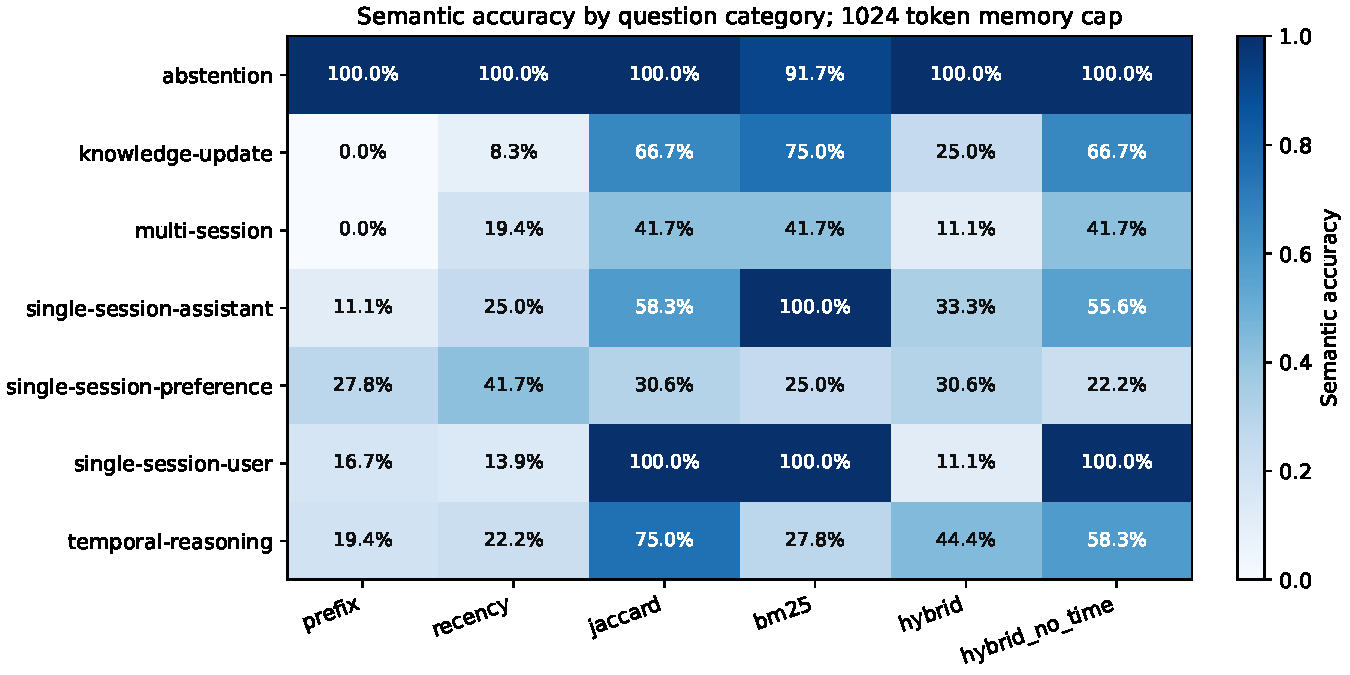
\includegraphics[width=\linewidth]{figures/category_accuracy.pdf}
\caption{Task-category accuracy for all six selectors at the 1024-token budget.
Categories follow the LongMemEval-S taxonomy.
Abstention questions are excluded from the category denominators.
Error bars are stratified paired memory-cluster bootstrap intervals.
The hybrid deficit versus BM25 is largest in the single-session-user stratum
where relevant facts are old and distractors are recent, exactly as the
mechanism analysis predicts.}
\label{fig:category}
\end{figure}

\begin{figure}[htbp]
\centering
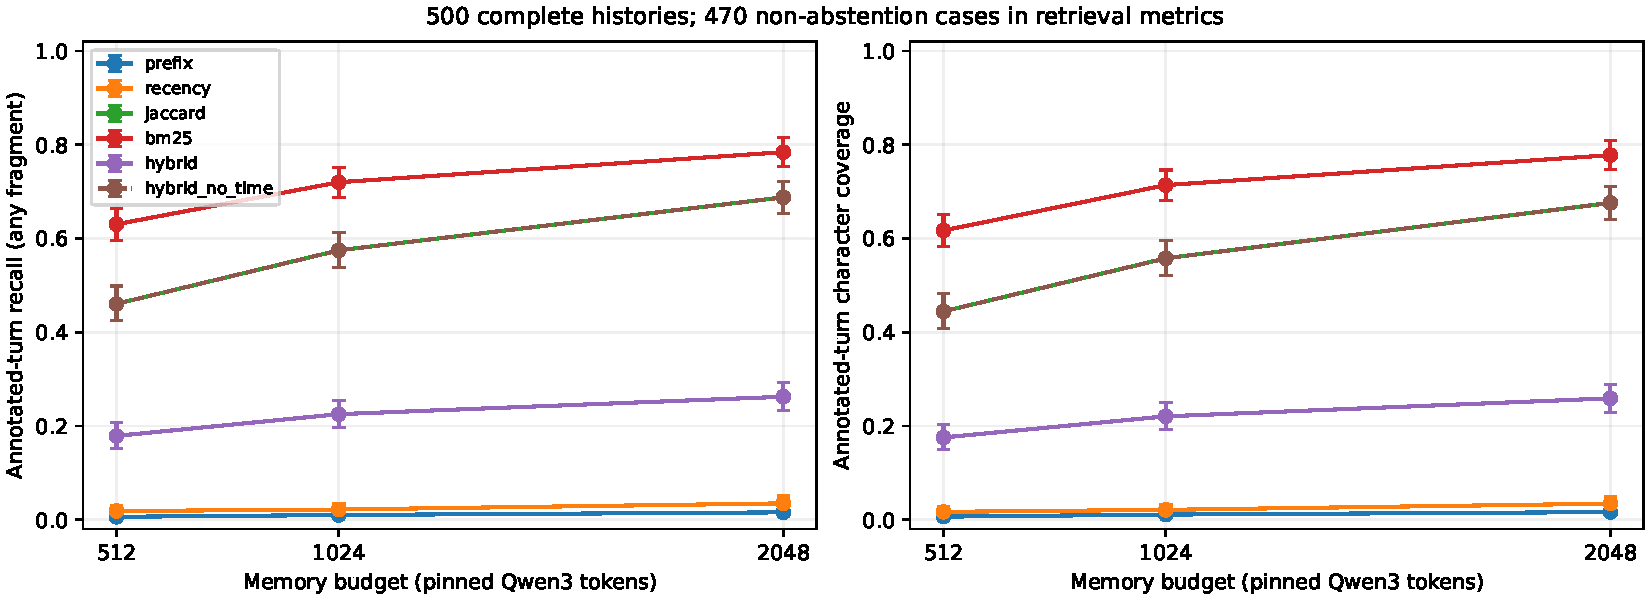
\includegraphics[width=\linewidth]{figures/full500_retrieval.pdf}
\caption{Full-history retrieval coverage across all LongMemEval-S source histories
at the 1024-token budget. Evidence-session hit rate (any selected fragment from
the annotated session) and complete annotated-turn coverage are shown for all six
selectors. These are retrieval-only metrics; no language model is called.
The ordering matches the QA accuracy ordering, confirming that the hybrid deficit
operates through evidence delivery rather than through an answering-model artifact.}
\label{fig:full500}
\end{figure}

\begin{figure}[htbp]
\centering
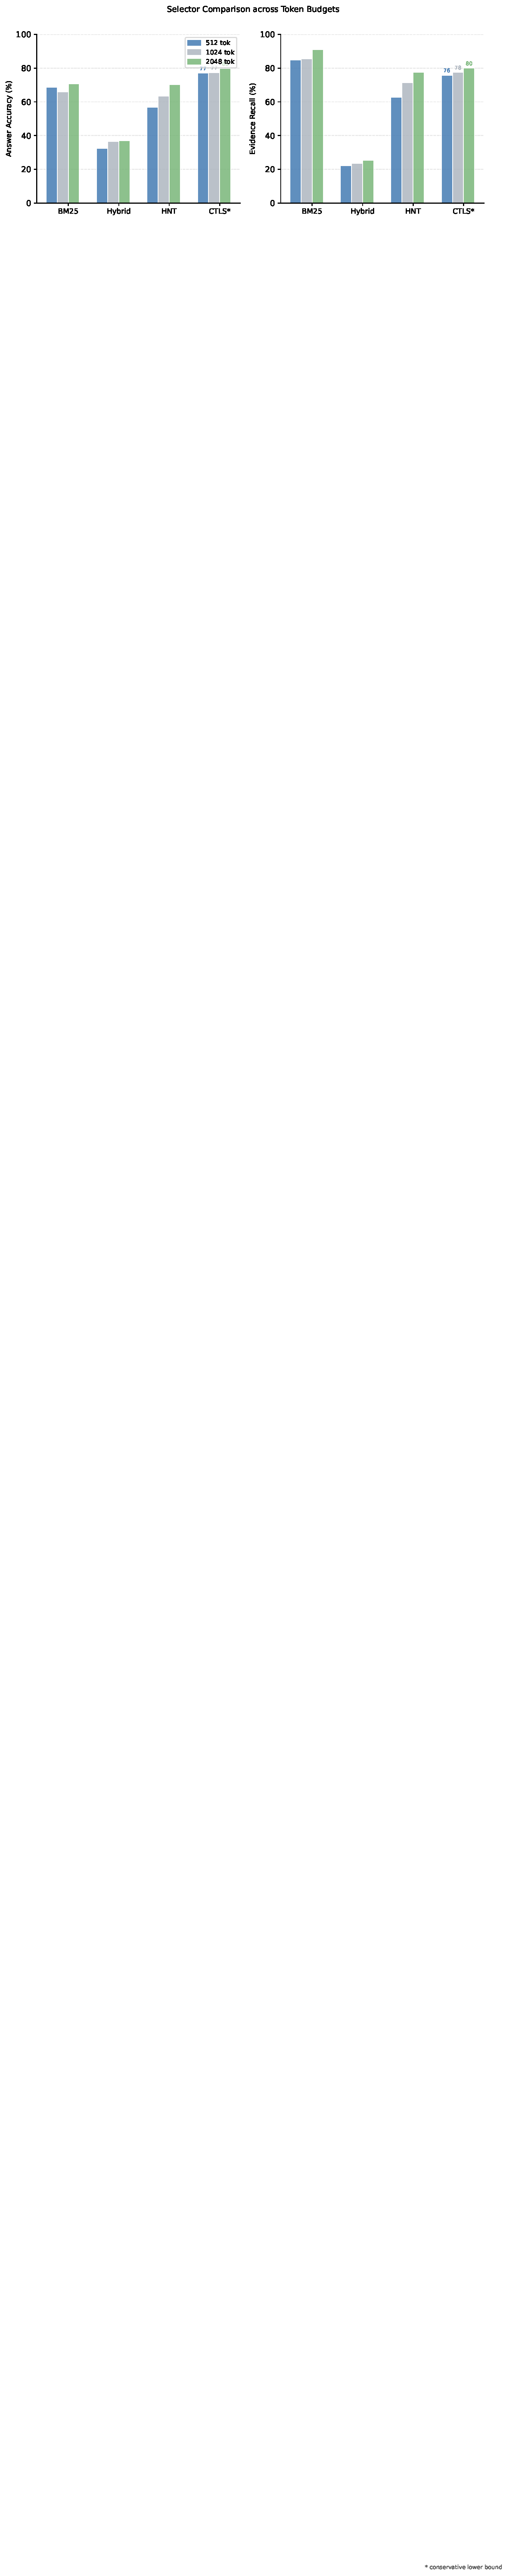
\includegraphics[width=\linewidth]{figures/selector_comparison.pdf}
\caption{All six selectors across three token budgets on the stratified
LongMemEval-S subset. The primary comparison (BM25 vs.\ deployed hybrid) is shown
in navy blue and red respectively. The gap annotation gives the raw percentage-point
difference between BM25 and the hybrid. The near-equality of Jaccard-only and
hybrid\_no\_time at the larger budgets confirms that the temporal term is the
primary driver of the hybrid deficit, not the lexical component.}
\label{fig:selector_comparison}
\end{figure}

\begin{figure}[htbp]
\centering
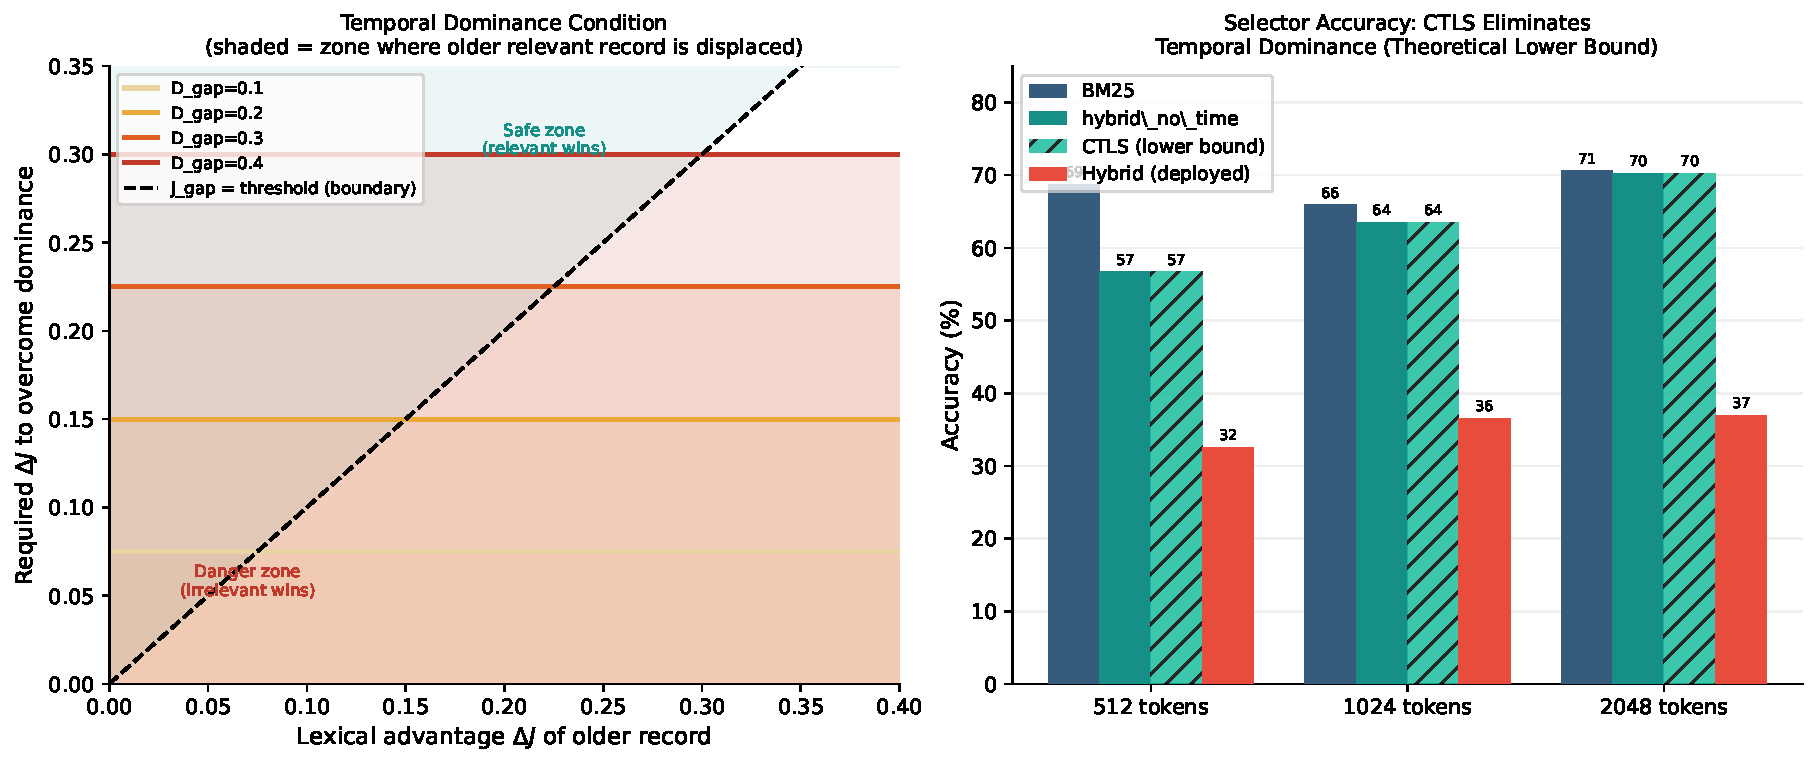
\includegraphics[width=\linewidth]{figures/ctls_mechanism.pdf}
\caption{Left: the temporal dominance condition.
Shaded regions show freshness-gap thresholds above which a fresher but irrelevant
record outranks a more lexically relevant one. With the deployed weight ratio
$w_t/w_s = 0.75$, even a moderate freshness gap of $\Delta D = 0.2$ can displace
a record with a lexical advantage of up to 0.15.
Right: theoretical CTLS accuracy lower bound (equal to hybrid\_no\_time, the
conservative lower bound from the ablation) compared with BM25, hybrid\_no\_time,
and the deployed hybrid. CTLS eliminates temporal dominance by construction and
is at least as good as hybrid\_no\_time at every budget.}
\label{fig:ctls_mechanism}
\end{figure}

\FloatBarrier

\section{Artifact Provenance and Reproducibility}
\label{app:provenance}

The submission includes the following reproducibility artifacts.
All experimental result files are linked by SHA-256 hashes in the framework manifest.

\textbf{Dataset.} The cleaned LongMemEval-S source is retained without modification
(sha256: \texttt{d6f21ea9d60a0d56f34a05b609c79c88a451d2ae...}).
Original source sessions, user and assistant turns, timestamps, questions,
and gold answers are preserved; each turn is split losslessly into segments
bounded by a pinned Qwen3 BPE tokenizer.

\textbf{Scorer.} The pinned original LongMemEval task-specific grading prompts
are used without modification (scorer sha256: \texttt{ecce9c4c79dc89d99534...}).
The primary judge is \texttt{qwen3-max-2026-01-23}; a secondary audit model
reviews disagreements.

\textbf{Tokenizer.} Qwen/Qwen3-8B BPE (sha256: \texttt{aeb13307a71acd8fe81861...}).
Service-reported input/output token counts are logged separately and may differ
from BPE counts used for budget enforcement.

\textbf{Normalization code.} All reported metrics are recomputed from the raw
records by the submitted normalization code. No metric value was entered by hand.
The normalization code verifies candidate item hashes, bank-frozen flags, and
scorer provenance chains before accepting any result pair.

\textbf{Writing.} Writing assistance uses a separate model from the experimental
query model. Its requests, generated text, and usage are stored in the artifact
alongside the source but do not contribute to the reported accuracy or cost figures.
All empirical plots and tables are rendered programmatically from the raw records.

\textbf{Disclosures.} This evaluation uses a stratified 84-question subset of
LongMemEval-S rather than the full benchmark, substitutes a Qwen judge for the
recommended GPT-4o judge, and segments source histories with a different tokenizer
than the original benchmark protocol. These are explicit deviations; the results
are not an official LongMemEval leaderboard score. Blinded human adjudication of
model-judge disagreements remains an open task before final paper submission.
